%!TEX root = thesis.tex

\chapter{Appendix}

\section{Detailed AI Use Cases in TinyML Research}
\label{app:detailed-ai-use-cases}

\begin{figure}[htbp]
    \centering
    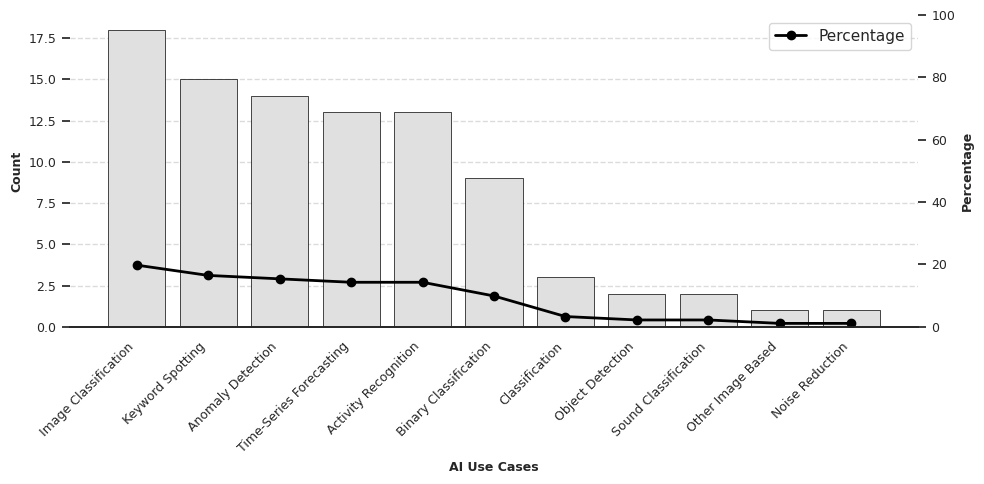
\includegraphics[width=0.98\textwidth]{figs/research_results/ai_use_case_detailed.png}
    \caption[Detailed AI Use Case Distribution]{Fine-grained distribution of AI use cases across the reviewed studies, showing the prevalence of specific applications such as image classification, keyword spotting, and anomaly detection.}
    \label{fig:detailed-ai-use-cases}
\end{figure}

\section{CI/CD Tactics and Optimization Techniques in TinyMLOps}
\label{app:cicd-optim-techniques}

\begin{table}[htbp]
    \centering
    \caption{CI/CD Tactics and Optimization Techniques in TinyMLOps}
    \label{tab:cicd-optim-techniques}
    \begin{tabularx}{\textwidth}{l l X}
        \toprule
        \textbf{Tactic / Technique} & \textbf{Category} & \textbf{Description} \\
        \midrule
        Full Model Update & CI/CD Tactic & Replaces the entire model on the device with a new version. Suitable for significant model changes or retraining. \\
        \midrule
        Partial Model Update & CI/CD Tactic & Updates only specific parts or layers of the model, reducing update size and deployment time. Useful for incremental improvements or fine-tuning. \\
        \midrule
        Automated Deployment & CI/CD Tactic & Automates the process of deploying new models to devices, ensuring efficient and consistent updates across fleets of devices. \\
        \midrule
        Automated Tests & CI/CD Tactic & Integrates automated testing into the CI/CD pipeline to validate model performance and system stability after updates. \\
        \midrule
        Quantization & Optimization Technique & Reduces model precision (e.g., from float32 to int8), decreasing model size and inference latency with minimal accuracy loss. \\
        \midrule
        Pruning & Optimization Technique & Removes less important weights or connections from the model, reducing model size and computational cost. \\
        \midrule
        Knowledge Distillation & Optimization Technique & Trains a smaller "student" model to mimic the behavior of a larger, more complex "teacher" model, transferring knowledge and improving efficiency. \\
        \midrule
        Feature Caching & Optimization Technique & Caches frequently used intermediate feature maps during inference to reduce redundant computations and improve latency. \\
        \midrule
        Adaptive Computation & Optimization Technique & Dynamically adjusts the computational workload based on input complexity or resource availability, optimizing energy consumption and latency. \\
        \midrule
        Test-Time Adaptation & Optimization Technique & Fine-tunes or adapts the model parameters during inference based on individual input samples or local data distributions, improving personalization and robustness to drift. \\
        \bottomrule
    \end{tabularx}
\end{table}
\clearpage

\section{H1 and H2 Evalauation Time Series Data}
\label{app:eval-data}

\begin{figure}[htbp]
    \centering
    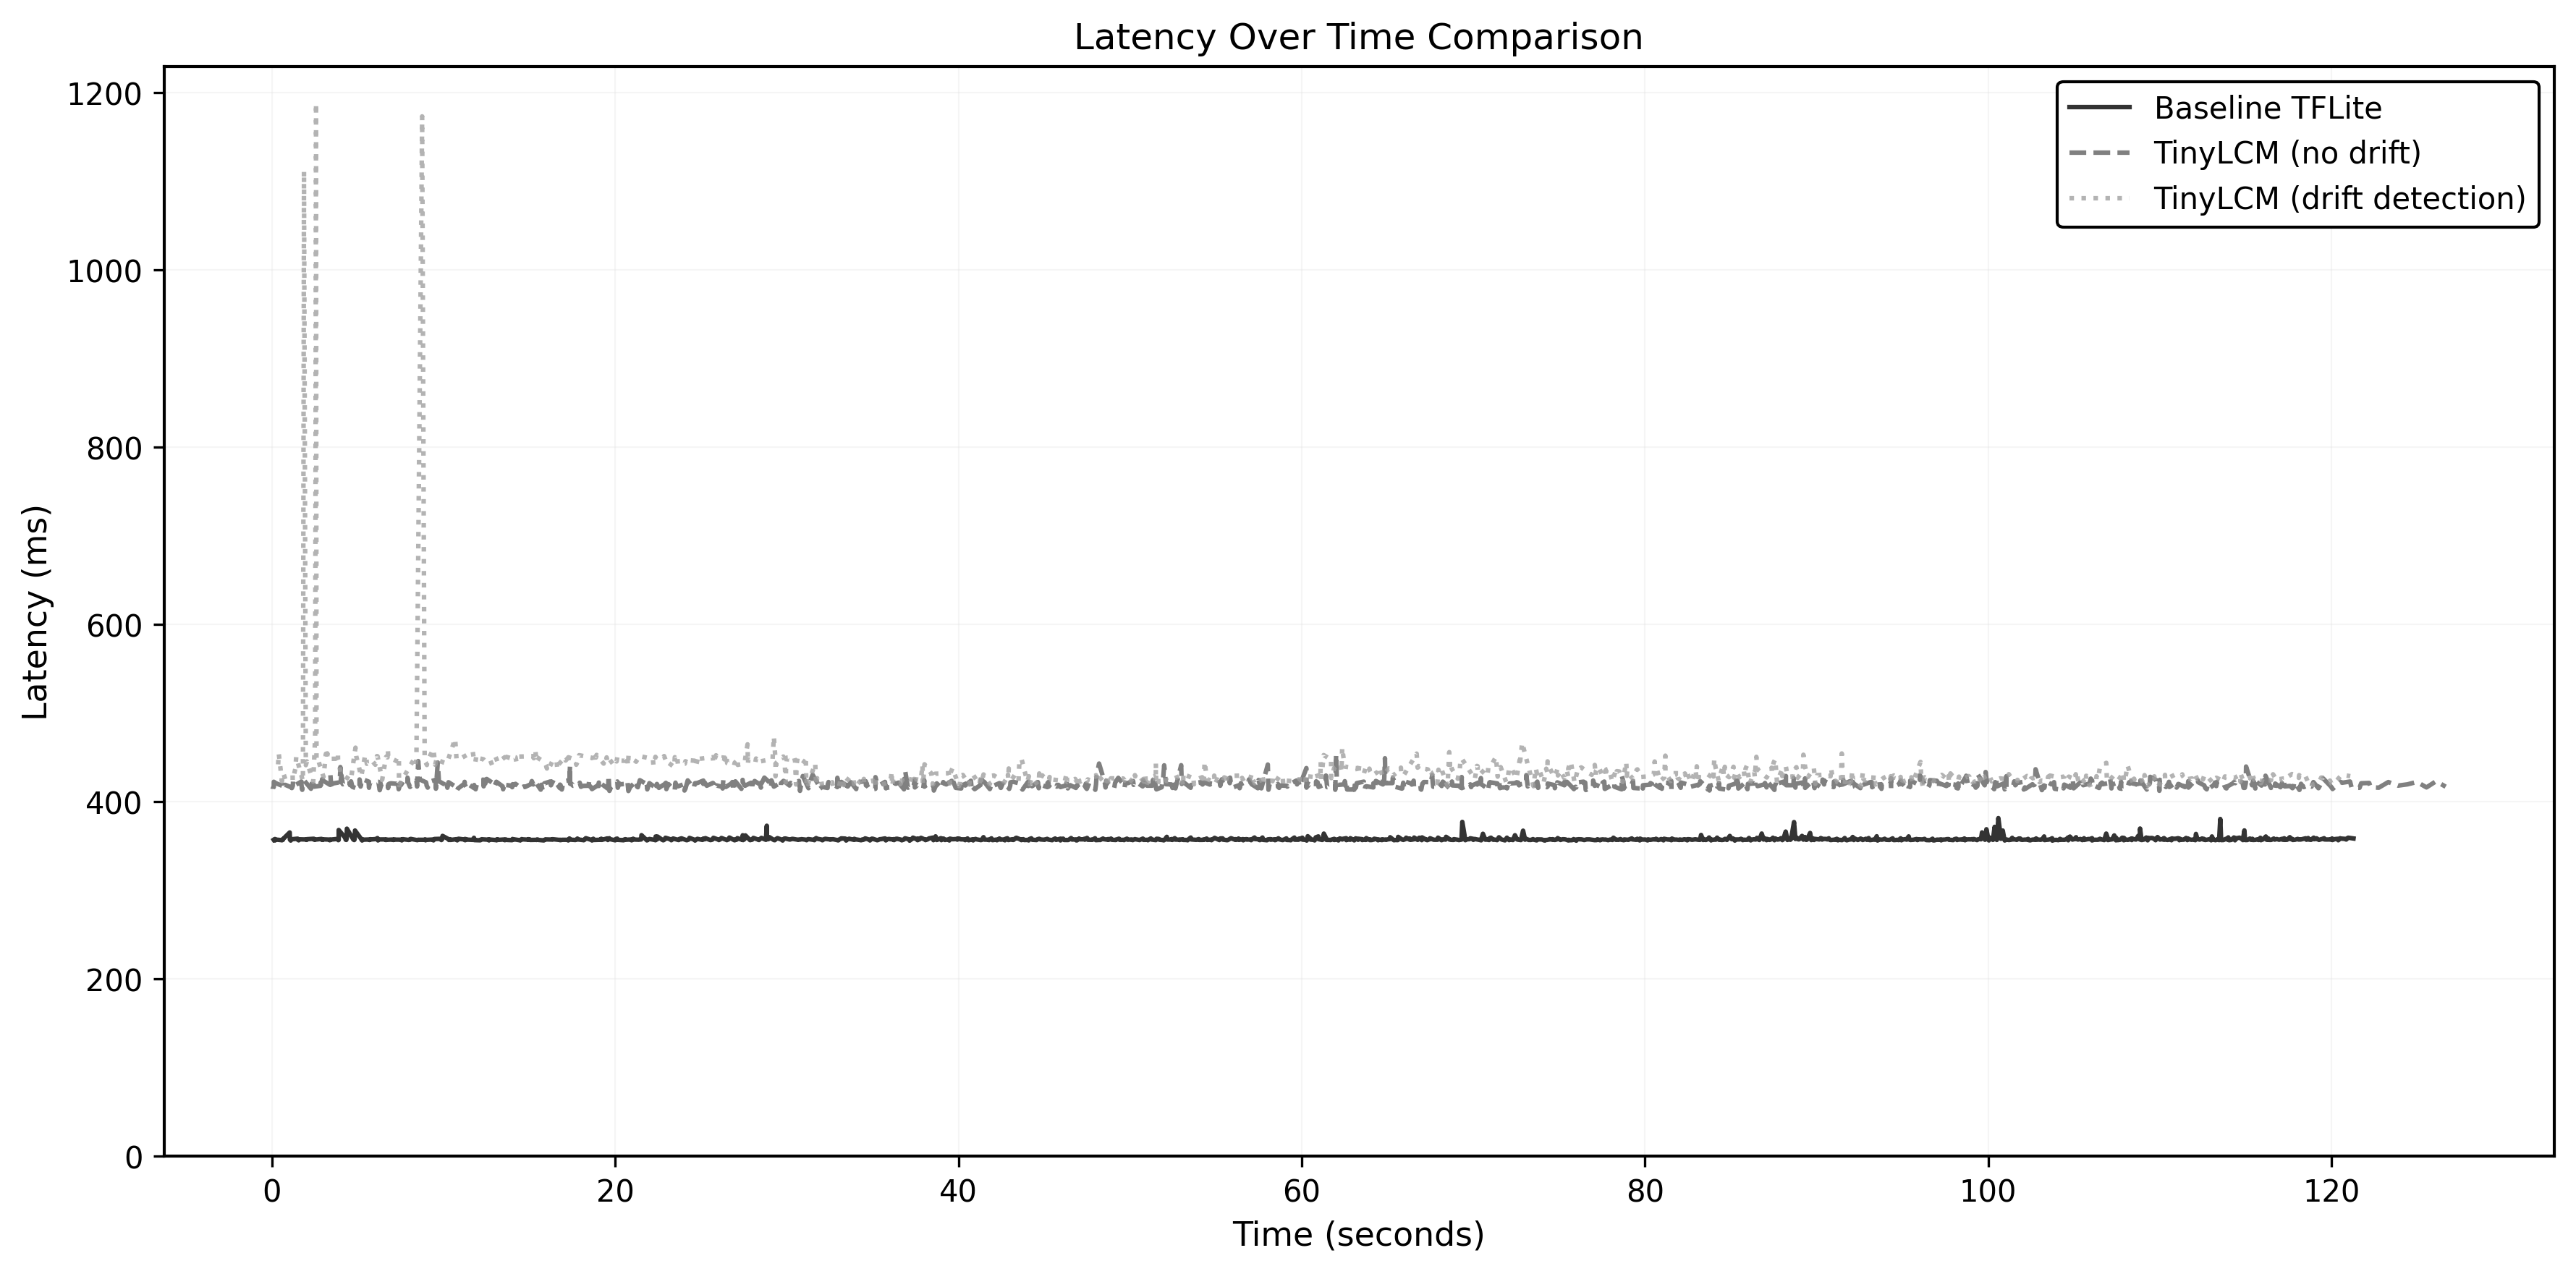
\includegraphics[width=0.98\textwidth]{figs/evaluation/latency_timeseries.png}
    \caption[Latency Comparison]{Time series diagram comparing the latency of the different approaches}
    \label{fig:latency-comparison}
\end{figure}

\begin{figure}[htbp]
    \centering
    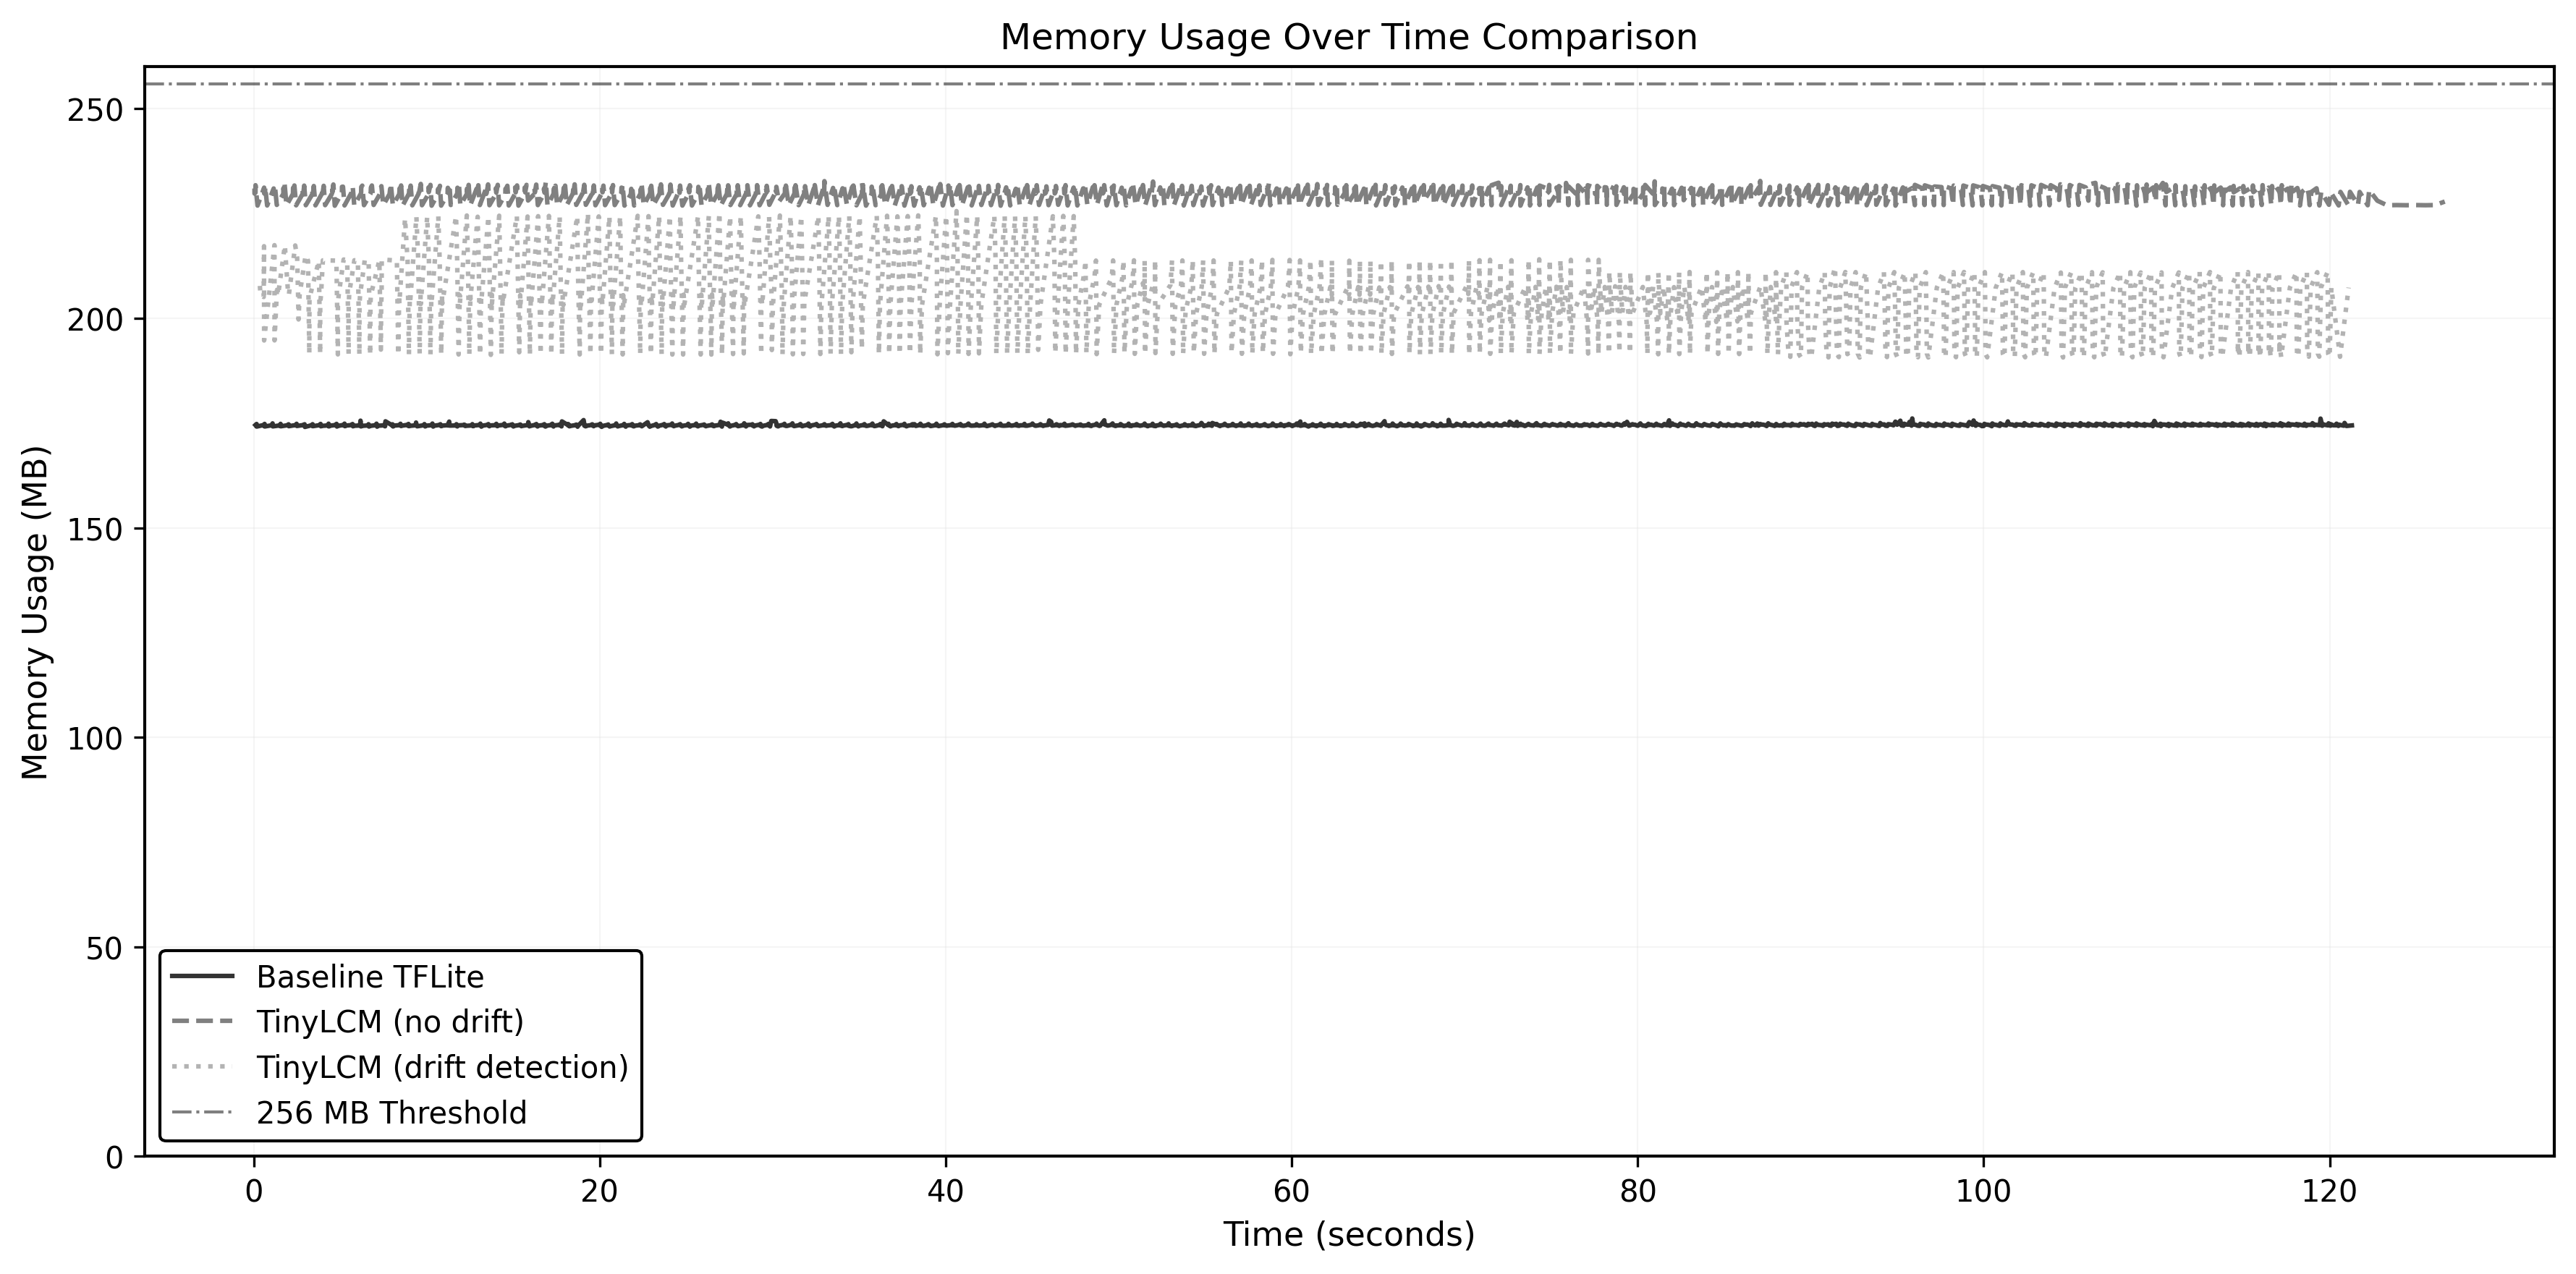
\includegraphics[width=0.98\textwidth]{figs/evaluation/memory_timeseries.png}
    \caption[Memory Comparison]{Time series diagram comparing memory usage of the different approaches}
    \label{fig:memory-comparison}
\end{figure}

\begin{figure}[htbp]
    \centering
    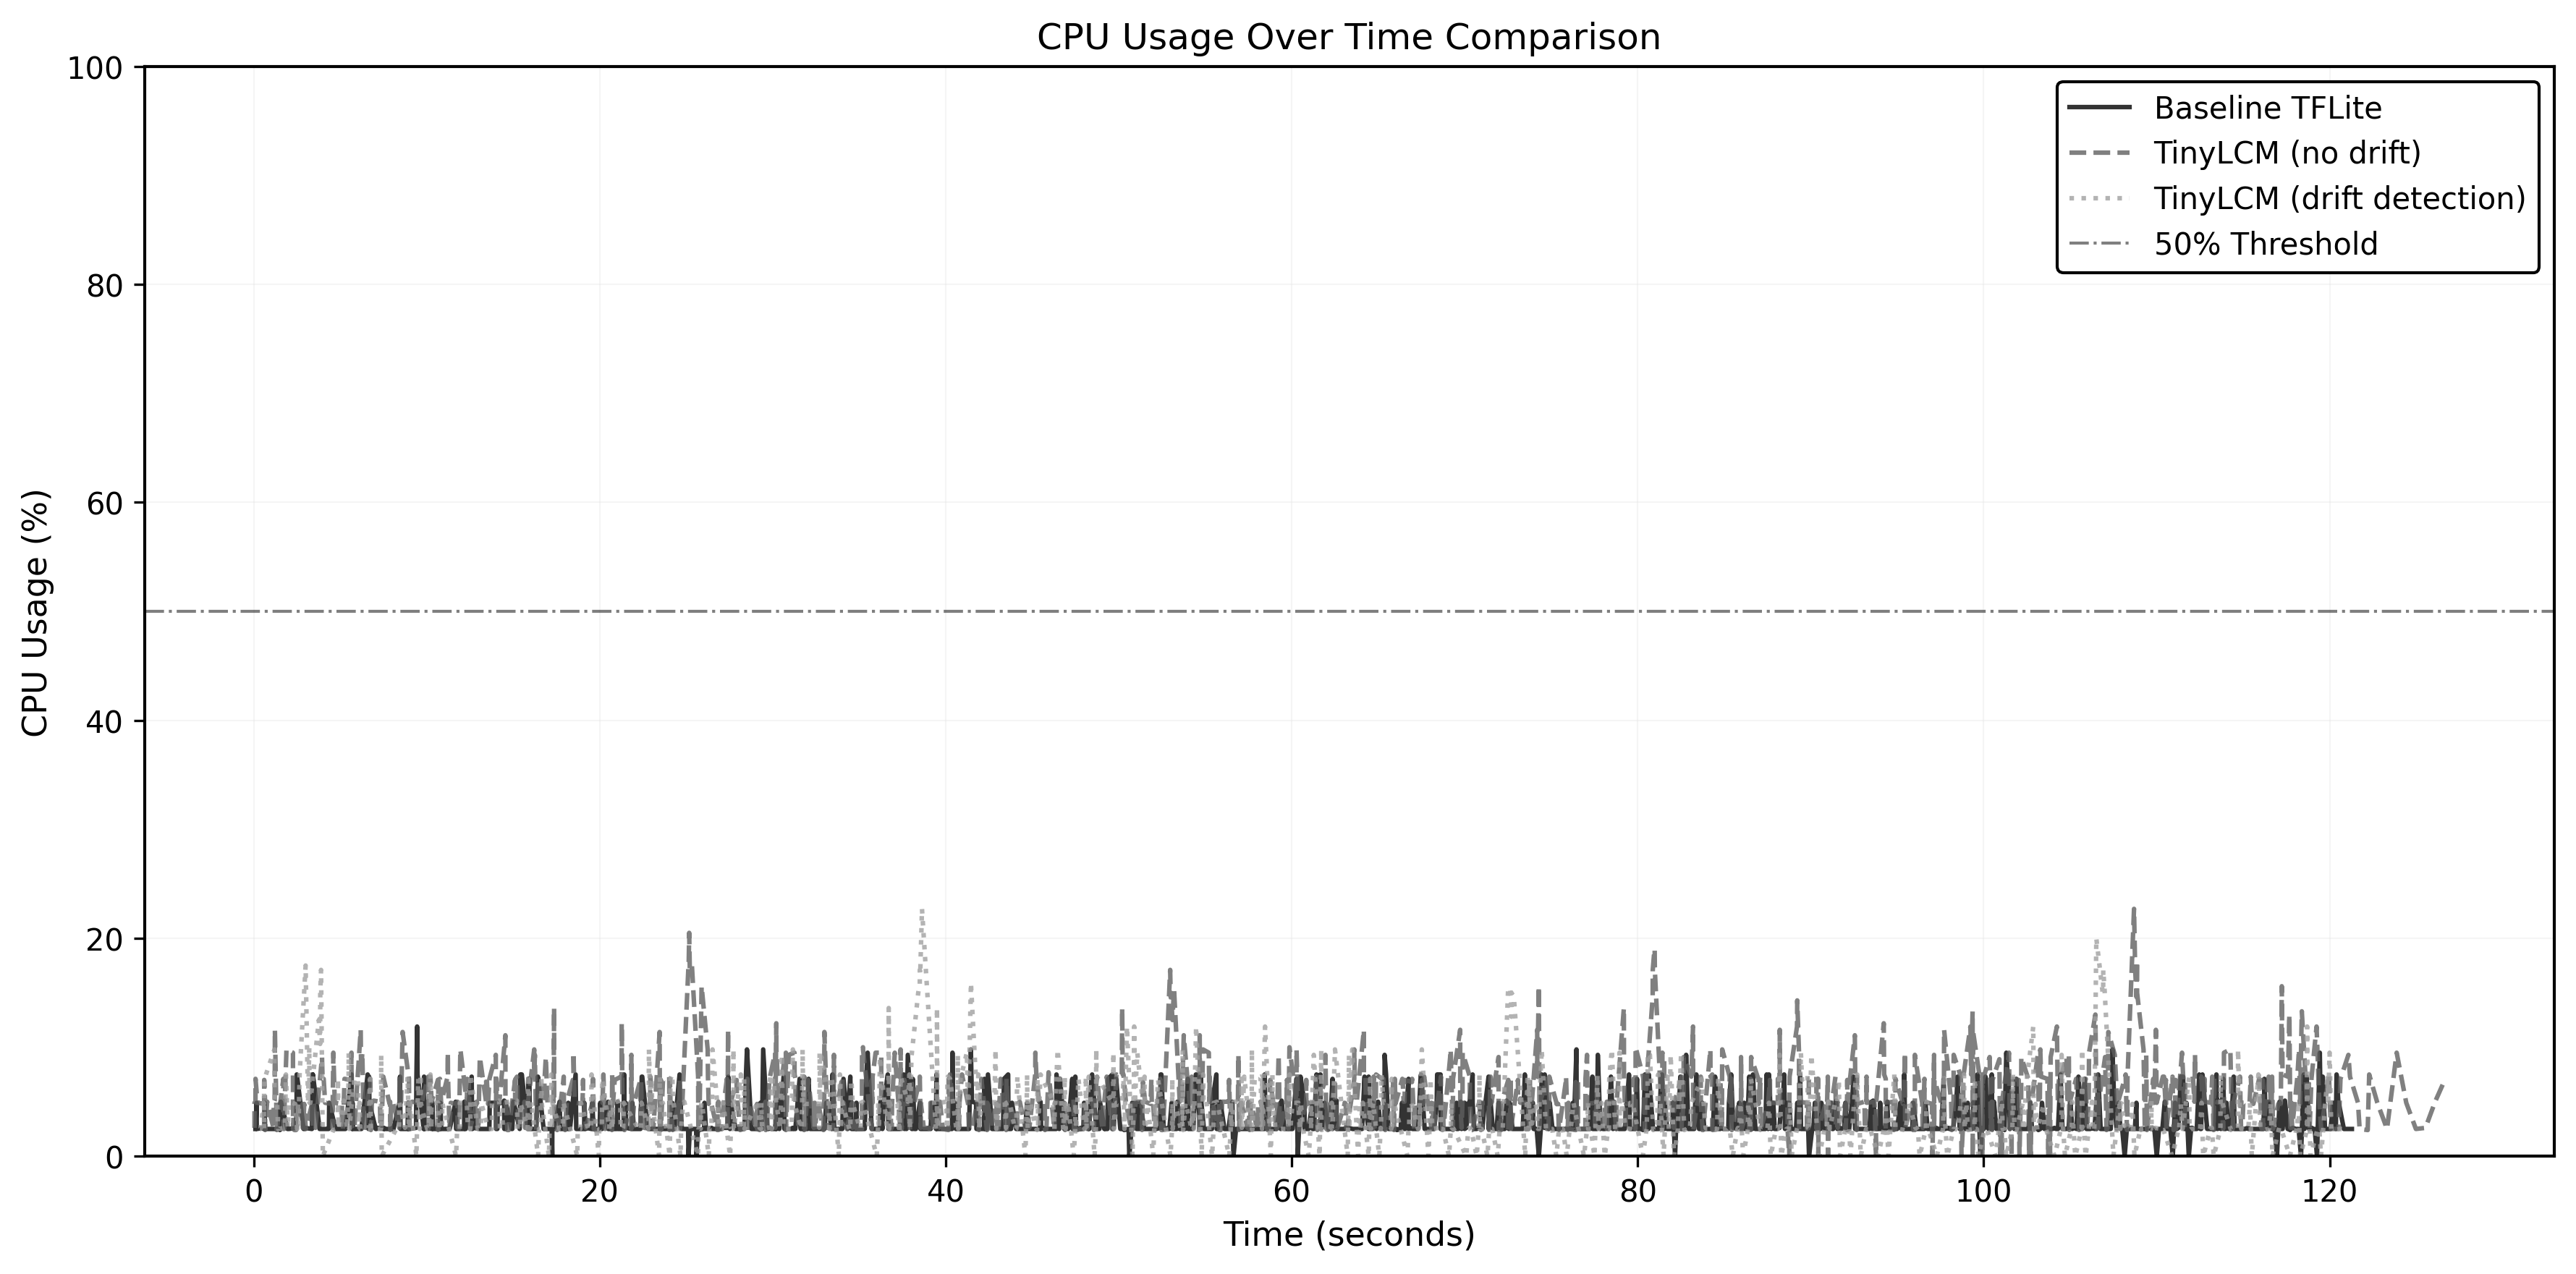
\includegraphics[width=0.98\textwidth]{figs/evaluation/cpu_timeseries.png}
    \caption[CPU Comparison]{Time series diagram comparing the CPU utilization of the different approaches.}
    \label{fig:cpu-comparison}
\end{figure}
